% !TEX program = pdflatex
%Numerical Experiment_1
\documentclass[10pt,a4paper]{article}
\usepackage[UTF8]{ctex}
\usepackage{bm}
\usepackage{amsmath}
\usepackage{amssymb}
\usepackage{graphicx}
\usepackage{geometry}
\geometry{a4paper,left=.3cm,right=.3cm,top=1cm,bottom=1.5cm}
\usepackage{multirow}
\usepackage{listings}
\usepackage[framed,numbered,autolinebreaks,useliterate]{mcode}
\usepackage{textcomp}
\title{数值试验一报告}
\author{陈稼霖 \and 45875852}
\date{2019.3.21}
\begin{document}
\maketitle
\section{问题的提出}
正方形区域上的泊松问题
\[
\left\{\begin{array}{l}
-(\frac{\partial^2x}{\partial x^2}+\frac{\partial^2u}{\partial y^2})=f(x,y),0<x,y<1,\\
u(0,y)=u(1,y)=u(x,0)=u(x,1)
\end{array}\right.
\]
取$f(x,y)=2\pi\sin(\pi x)\sin(\pi y)$,问题的精确解为$u^*(x,y)=\sin(\pi x)\sin(\pi y)$. 将正方形区域平均划分为$N\times N$个小方格,方程组的差分格式为
\[
\left\{\begin{array}{l}
-u_{i-1,j}-u_{i,j-1}+4u_{i,j}-u_{i+1,j}-u_{i,j+1}=h^2f_{i,j}\\
u_{0,j}=u_{N,j}=u_{i,0}=u_{i,N}
\end{array}\right.
\]
记
\begin{gather*}
u_j^h=\left(\begin{array}{l}
u_{1,j}\\
u_{2,j}\\
\vdots\\
u_{N-1,j}
\end{array}\right),
f_j^h=\left(\begin{array}{l}
f_{1,j}\\
f_{2,j}\\
\vdots\\
f_{N-1,j}
\end{array}\right),
u^h=\left(\begin{array}{l}
u_1^h\\
u_2^h\\
\vdots\\
u_{N-1}^h
\end{array}\right),
f^h=\left(\begin{array}{l}
f_1^h\\
f_2^h\\
\vdots\\
f_{N-1}^h
\end{array}\right),\\
C=\left(\begin{array}{cccccc}
0 & 1 &    &    &    &\\
1 & 0 & 1 &    &    &\\
   & 0 & 1 & 0 &    &\\
   &    & \ddots & \ddots & \ddots &\\
   &    &    & 1 & 0 & 1\\
   &    &    &    & 1 & 0\\
\end{array}\right),
L_h=\left(\begin{array}{cccccc}
4I-C & -I &    &    &    &\\
-I & 4I-C & -I &    &    &\\
   & \ddots & \ddots & \ddots & &\\
   &    &    & -I & 4I-C & -I\\
   &    &    &    & -I & 4I-C\\
\end{array}\right)
\end{gather*}
其中$I$为$N-1$阶单位矩阵. 将差分格式写为
\begin{equation}
\label{equsys}
L_hu^h=h^2f^h
\end{equation}
\section{数值试验}
1. 取$h=0.1$,分析用不同迭代法求解方程组(\ref{equsys})的收敛性,并求出使$||u^{(k+1)}-u^{(k)}||<\varepsilon$的近似解及相应的迭代次数,其中$u^{(k)}$为求解(\ref{equsys})的第$k$次迭代解,$\varepsilon=10^{-6}$. 并与精确解$u^*$做比较. 考虑用(1)雅可比迭代法;(2)赛德尔迭代法;(3)超松弛迭代法($\omega$取$1.2$,$1.3$,$1.9$,$0.9$).\\
(本次实验均以$u^{(k)}=ones((N - 1)^2,1)$为初始向量进行迭代)\\
(1)雅可比迭代法求出的近似解:
\tiny
\begin{align*}
u^{(k)}=&\\
[&0.096282596713267,0.183140370210779,0.252071110720433,0.296327343713280,0.311577028014331,0.296327343713280,0.252071110720433,0.183140370210779,0.096282596713267,\\
&0.183140370210779,0.348353707433701,0.479467713924059,0.563648138734764,0.592654687426560,0.563648138734765,0.479467713924059,0.348353707433701,0.183140370210779,\\
&0.252071110720433,0.479467713924059,0.659930735448032,0.775795057637339,0.815719249455198,0.775795057637339,0.659930735448032,0.479467713924059,0.252071110720433,\\
&0.296327343713280,0.563648138734764,0.775795057637339,0.912001846168465,0.958935427848119,0.912001846168465,0.775795057637339,0.563648138734765,0.296327343713280,\\
&0.311577028014331,0.592654687426560,0.815719249455198,0.958935427848119,1.008284442881733,0.958935427848119,0.815719249455198,0.592654687426560,0.311577028014331,\\
&0.296327343713280,0.563648138734764,0.775795057637339,0.912001846168465,0.958935427848119,0.912001846168465,0.775795057637339,0.563648138734764,0.296327343713280,\\
&0.252071110720433,0.479467713924059,0.659930735448032,0.775795057637339,0.815719249455198,0.775795057637339,0.659930735448032,0.479467713924059,0.252071110720433,\\
&0.183140370210779,0.348353707433701,0.479467713924059,0.563648138734765,0.592654687426560,0.563648138734765,0.479467713924060,0.348353707433701,0.183140370210779,\\
&0.096282596713267,0.183140370210779,0.252071110720433,0.296327343713280,0.311577028014331,0.296327343713280,0.252071110720433,0.183140370210779,0.096282596713267]^T
\end{align*}
\normalsize
(2)赛德尔迭代法求出的近似解:
\tiny
\begin{align*}
u^{(k)}=&\\
[&0.096282095014263,0.183139305299849,0.252069468476958,0.296325253065745,0.311574630504295,0.296324920581546,0.252068902108678,0.183138686768656,0.096281660166459,\\
&0.183139305299849,0.348351437909015,0.479464331185244,0.563643801598307,0.592649841163039,0.563643200128708,0.479463306615346,0.348350318975516,0.183138518652742,\\
&0.252069468476958,0.479464331185244,0.659925657440196,0.775788713795995,0.815712102237337,0.775787926462024,0.659924316260711,0.479462866482196,0.252068438742469,\\
&0.296325253065745,0.563643801598307,0.775788713795995,0.911993855335958,0.958926613230658,0.911992975069768,0.775787214311661,0.563642164010424,0.296324101787522,\\
&0.311574630504295,0.592649841163039,0.815712102237337,0.958926613230658,1.008274635236227,0.958925732964420,0.815710602752922,0.592648203575069,0.311573479226012,\\
&0.296324920581546,0.563643200128708,0.775787926462024,0.911992975069768,0.958925732964420,0.911992178861438,0.775786570165566,0.563641718916405,0.296323879240509,\\
&0.252068902108678,0.479463306615346,0.659924316260711,0.775787214311661,0.815710602752922,0.775786570165566,0.659923218993784,0.479462108289375,0.252068059646051,\\
&0.183138686768656,0.348350318975516,0.479462866482197,0.563642164010424,0.592648203575069,0.563641718916405,0.479462108289375,0.348349490952611,0.183138104641281,\\
&0.096281660166459,0.183138518652742,0.252068438742469,0.296324101787522,0.311573479226012,0.296323879240509,0.252068059646050,0.183138104641281,0.096281369102766]^T
\end{align*}
\normalsize
(3)超松弛迭代法求出的近似解:\\
当$\omega=1.2$时,
\tiny
\begin{align*}
u^{(k)}=&\\
[&0.096281691354415,0.183138530015131,0.252068396247185,0.296323991888770,0.311573308644520,0.296323671559953,0.252067849617325,0.183137931278956,0.096281268689381,\\
&0.183138530015131,0.348349956123932,0.479462290558075,0.563641410331563,0.592647343119902,0.563640846686530,0.479461328717649,0.348348902598140,0.183137786301063,\\
&0.252068396247185,0.479462290558075,0.659922857696348,0.775785443815110,0.815708696303852,0.775784726156341,0.659921633036897,0.479460949160599,0.252067449316242,\\
&0.296323991888770,0.563641410331563,0.775785443815110,0.911990047386572,0.958922657435296,0.911989266945657,0.775784112020136,0.563639951586101,0.296322962118517,\\
&0.311573308644520,0.592647343119902,0.815708696303852,0.958922657435296,1.008270535635037,0.958921898321200,0.815707400902344,0.592645924237035,0.311572307014415,\\
&0.296323671559953,0.563640846686530,0.775784726156341,0.911989266945657,0.958921898321200,0.911988599083657,0.775783586473327,0.563639598365687,0.296322790334472,\\
&0.252067849617325,0.479461328717649,0.659921633036897,0.775784112020136,0.815707400902344,0.775783586473327,0.659920736209750,0.479460346402385,0.252067156172811,\\
&0.183137931278956,0.348348902598140,0.479460949160599,0.563639951586101,0.592645924237035,0.563639598365687,0.479460346402385,0.348348242383297,0.183137465214366,\\
&0.096281268689381,0.183137786301063,0.252067449316242,0.296322962118517,0.311572307014415,0.296322790334472,0.252067156172811,0.183137465214366,0.096281042025073]^T
\end{align*}
\normalsize
当$\omega=1.3$时,
\tiny
\begin{align*}
u^{(k)}=&\\
[&0.096281632281658,0.183138393233463,0.252068181194723,0.296323714523445,0.311572997474069,0.296323362182267,0.252067578754821,0.183137731212908,0.096281162818419,\\
&0.183138393233463,0.348349658928740,0.479461841771555,0.563640847418933,0.592646724364534,0.563640241019561,0.479460804937937,0.348348519553402,0.183137585260307,\\
&0.252068181194723,0.479461841771555,0.659922198626763,0.775784633853820,0.815707819774381,0.775783878662965,0.659920907386530,0.479460422829064,0.252067174970167,\\
&0.296323714523445,0.563640847418933,0.775784633853820,0.911989067396832,0.958921609875873,0.911988264121513,0.775783260397822,0.563639338129627,0.296322644230624,\\
&0.311572997474069,0.592646724364534,0.815707819774381,0.958921609875873,1.008269426939931,0.958920845658129,0.815706513099794,0.592645288461249,0.311571979221987,\\
&0.296323362182267,0.563640241019561,0.775783878662965,0.911988264121513,0.958920845658128,0.911987606490231,0.775782754232017,0.563639005383613,0.296322485947155,\\
&0.252067578754821,0.479460804937937,0.659920907386530,0.775783260397822,0.815706513099794,0.775782754232017,0.659920041934245,0.479459853893360,0.252066904333966,\\
&0.183137731212908,0.348348519553402,0.479460422829064,0.563639338129627,0.592645288461249,0.563639005383613,0.479459853893360,0.348347894350573,0.183137287858479,\\
&0.096281162818419,0.183137585260307,0.252067174970167,0.296322644230624,0.311571979221987,0.296322485947155,0.252066904333966,0.183137287858479,0.096280951919793]^T
\end{align*}
\normalsize
当$\omega=1.9$时,
\tiny
\begin{align*}
u^{(k)}=&\\
[&0.096280584835522,0.183136896642189,0.252066175973691,0.296321505822835,0.311571541561488,0.296321398037666,0.252066645860813,0.183136912720906,0.096280744728857,\\
&0.183136896642189,0.348346870551354,0.479458184617037,0.563637578832648,0.592643350834964,0.563637385361955,0.479458684582322,0.348347059033324,0.183137070049542,\\
&0.252066175973690,0.479458184617037,0.659918444197920,0.775780071052998,0.815704206009224,0.775780283367984,0.659918237513913,0.479458824823702,0.252066456181786,\\
&0.296321505822835,0.563637578832648,0.775780071052998,0.911984757747605,0.958917595801752,0.911984510733432,0.775780517933801,0.563637807820625,0.296322018990652,\\
&0.311571541561488,0.592643350834964,0.815704206009224,0.958917595801752,1.008265913795882,0.958917504473366,0.815704187692265,0.592644097866816,0.311571472038355,\\
&0.296321398037666,0.563637385361955,0.775780283367983,0.911984510733432,0.958917504473366,0.911984513206622,0.775780424012973,0.563637667788378,0.296321627057609,\\
&0.252066645860813,0.479458684582322,0.659918237513913,0.775780517933801,0.815704187692265,0.775780424012973,0.659918299451593,0.479458828454800,0.252066473940547,\\
&0.183136912720906,0.348347059033324,0.479458824823702,0.563637807820625,0.592644097866815,0.563637667788378,0.479458828454801,0.348347617018303,0.183137232782245,\\
&0.096280744728857,0.183137070049542,0.252066456181786,0.296322018990652,0.311571472038355,0.296321627057609,0.252066473940547,0.183137232782244,0.096280630157131]^T
\end{align*}
\normalsize
当$\omega=0.9$时,
\tiny
\begin{align*}
u^{(k)}=&\\
[&0.096282272681564,0.183139652398577,0.252069956791081,0.296325837342726,0.311575253471145,0.296325519388657,0.252069415406956,0.183139061575778,0.096281857729140,\\
&0.183139652398577,0.348352112742520,0.479465276565224,0.563644928555881,0.592651038777218,0.563644347898518,0.479464287873116,0.348351033764009,0.183138894599879,\\
&0.252069956791081,0.479465276565224,0.659926976905088,0.775790281493278,0.815713763305381,0.775789514170431,0.659925670375469,0.479463850724592,0.252068955380802,\\
&0.296325837342726,0.563644928555881,0.775790281493278,0.911995712466478,0.958928575746166,0.911994846410339,0.775788806849324,0.563643319248879,0.296324707078561,\\
&0.311575253471145,0.592651038777218,0.815713763305381,0.958928575746166,1.008276704139478,0.958927701449238,0.815712274629742,0.592649414157174,0.311574112452177,\\
&0.296325519388657,0.563644347898518,0.775789514170431,0.911994846410339,0.958927701449238,0.911994048076557,0.775788154838133,0.563642864433324,0.296324477506940,\\
&0.252069415406956,0.479464287873116,0.659925670375469,0.775788806849324,0.815712274629742,0.775788154838133,0.659924560188363,0.479463076304811,0.252068564486510,\\
&0.183139061575778,0.348351033764009,0.479463850724592,0.563643319248879,0.592649414157173,0.563642864433324,0.479463076304811,0.348350188624973,0.183138468009505,\\
&0.096281857729140,0.183138894599879,0.252068955380801,0.296324707078561,0.311574112452177,0.296324477506940,0.252068564486510,0.183138468009505,0.096281558122037]^T
\end{align*}
\normalsize
精确解:
\tiny
\begin{align*}
u^*=&\\
[&0.095491502812526,0.181635632001340,0.250000000000000,0.293892626146237,0.309016994374947,0.293892626146237,0.250000000000000,0.181635632001340,0.095491502812526,\\
&0.181635632001340,0.345491502812526,0.475528258147577,0.559016994374947,0.587785252292473,0.559016994374947,0.475528258147577,0.345491502812526,0.181635632001340,\\
&0.250000000000000,0.475528258147577,0.654508497187474,0.769420884293813,0.809016994374947,0.769420884293813,0.654508497187474,0.475528258147577,0.250000000000000,\\
&0.293892626146237,0.559016994374947,0.769420884293813,0.904508497187474,0.951056516295154,0.904508497187474,0.769420884293813,0.559016994374948,0.293892626146237,\\
&0.309016994374947,0.587785252292473,0.809016994374947,0.951056516295154,1.000000000000000,0.951056516295154,0.809016994374947,0.587785252292473,0.309016994374948,\\
&0.293892626146237,0.559016994374947,0.769420884293813,0.904508497187474,0.951056516295154,0.904508497187474,0.769420884293813,0.559016994374948,0.293892626146237,\\
&0.250000000000000,0.475528258147577,0.654508497187474,0.769420884293813,0.809016994374947,0.769420884293813,0.654508497187474,0.475528258147577,0.250000000000000,\\
&0.181635632001340,0.345491502812526,0.475528258147577,0.559016994374948,0.587785252292473,0.559016994374948,0.475528258147577,0.345491502812526,0.181635632001340,\\
&0.095491502812526,0.181635632001340,0.250000000000000,0.293892626146237,0.309016994374948,0.293892626146237,0.250000000000000,0.181635632001340,0.095491502812526]^T
\end{align*}
\normalsize
\begin{table}[h]
\centering\scriptsize
\caption{各迭代方法求解结果比较}
\begin{tabular}{|c|c|c|c|c|c|c|}\hline
\multirow{2}{*}{迭代方法} & \multirow{2}{*}{雅可比迭代法} & \multirow{2}{*}{赛德尔迭代法} & \multicolumn{4}{c|}{超松弛迭代法} \\ \cline{4-7} 
& & & $\omega=1.2$ & $\omega=1.3$ & $\omega=1.9$ & $\omega=0.9$\\ \hline
迭代次数$k$ & $206$ & $111$ & $76$ & $61$ & $134$ & $134$\\ \hline
\begin{tabular}[c]{@{}c@{}}与精确解之差的\\ 1-范数$||u^{(k)}-u^*||_1$\end{tabular} & $0.330245247376266$ & $0.329859823983780$ & $0.329697874010542$ & $0.329655405892316$ & $0.329491803895450$ & $0.329941467263010$\\ \hline
\begin{tabular}[c]{@{}c@{}}与精确解之差的\\ 2-范数$||u^{(k)}-u^*||_2$\end{tabular} & $0.041422051869794$ & $0.041373556852615$ & $0.041353189819760$ & $0.041347799507484$ & $0.041327525203464$ & $0.041383827166218$\\ \hline
\begin{tabular}[c]{@{}c@{}}与精确解之差的\\ $\infty$-范数$||u^{(k)}-u^*||_{\infty}$\end{tabular} & $0.008284442881733$ & $0.008274635236227$ & $0.008270535635037$ & $0.008269426939931$ & $0.008265913795882$ & $0.008276704139478$\\ \hline
\end{tabular}
\end{table}
\\从中可以看出,收敛速度:雅可比迭代$<$赛德尔迭代$<$超松弛因子迭代法(当选取合适的松弛因子),而与精确解的差距没有明显差距。

2. 用雅可比迭代法,分析$h$取不同值时,求解(\ref{equsys})的收敛情况,求出使$||u^{(k+1)-u^{(k)}}||<\varepsilon$的近似解及相应的迭代次数. 已知雅可比矩阵为$T=I-\frac{1}{4}L_h$,其谱半径为$\rho(T)=1-2\sin^2\frac{\pi h}{2}\approx1-\frac{\pi^2h^2}{2}$.\\
\begin{table}[h]
\centering\tiny
\caption{不同$h$(部分)下雅可比迭代法求解结果比较}
\begin{tabular}{|c|c|c|c|c|c|}\hline
$h$ & $0.01$ & $0.02$ & $0.05$ & $0.1$ & $0.2$\\ \hline
迭代次数$k$ & $11600$ & $3602$ & $722$ & $206$ & $55$\\ \hline
\begin{tabular}[c]{@{}c@{}}与精确解之差的\\ 1-范数$||u^{(k)}-u^*||_1$\end{tabular} & $0.330245247376266$ & $0.329859823983780$ & $0.329697874010542$ & $0.329655405892316$ & $0.329491803895450$\\ \hline
\begin{tabular}[c]{@{}c@{}}与精确解之差的\\ 2-范数$||u^{(k)}-u^*||_2$\end{tabular} & $0.041422051869794$ & $0.041373556852615$ & $0.041353189819760$ & $0.041347799507484$ & $0.041327525203464$\\ \hline
\begin{tabular}[c]{@{}c@{}}与精确解之差的\\ $\infty$-范数$||u^{(k)}-u^*||_{\infty}$\end{tabular} & $0.008284442881733$ & $0.008274635236227$ & $0.008270535635037$ & $0.008269426939931$ & $0.008265913795882$\\\hline
\end{tabular}
\end{table}
\\从中可以看出,随着$h$的减小,迭代次数急剧上升。

3. 简单阐述上述数值结果。\\
(1)关于三种迭代法收敛速度:雅可比迭代公式的分量形式为
\[
x_i^{(k+1)}=\frac{1}{a_{ii}}(b_i-\sum_{j\neq i}^na_{ij}x_j^{(k)}),~~i=1,2,...,n
\]
可见,雅可比迭代法完全通过前一迭代得到的$x^{(k)}$的各分量进行后一次迭代运算;\\
赛德尔迭代公式的分量形式为
\begin{equation}
\label{GS}
x_i^{(k+1)}=\frac{1}{a_{ii}}(b_i-\sum_{j=1}^{i-1}a_{ij}x_j^{(k+1)}-\sum_{j=i+1}^na_{ij}x_j^{(k)}),~~i=1,2,...,n
\end{equation}
可见,赛德尔迭代法在进行后一次迭代运算时,一部分用的是前一迭代得到的$x^{(k)}$的分量(式(\ref{GS})中第三项),另一部分用的是后一次迭代中已经算出的分量(式(\ref{GS})中第二项),因此赛德尔迭代法相比雅可比迭代法能更有快地逼近满足迭代终止条件的近似解;\\
而超松弛迭代公式的分量形式为
\begin{gather*}
\widetilde{x}_i^{(k+1)}=\frac{1}{a_{ii}}(b_i-\sum_{i=1}^{i-1}a_{ij}x_j^{(k+1)}-\sum_{j=i+1}^na_{ij}x_j^{(k)})\\
x_i^{(k+1)}=(1-\omega)x_i^{(k)}+\omega\widetilde{x}_i^{(k+1)}
\end{gather*}
可见,超松弛迭代法将用赛德尔迭代法计算出来的后一次迭代计算结果和前一次迭代计算结果的加权平均作为其后一次迭代的计算结果,当选取适当的权值$\omega$(也就是松弛因子),可以得到合适的收敛步长,从而避免“收敛过头”(比如前一步迭代得到的近似值大于精确值,但由于收敛步长过大,导致后一步迭代得到的近似值小于精确值,近似值在精确值附近来回波动,但不靠近精确值,这样一来会导致需要迭代多次才能达到终止迭代的条件),因此超松弛迭代法相比赛德尔迭代法能更有效率地逼近满足迭代终止条件的近似解。\\
(2)关于不同$h$下雅可比迭代法收敛速度:随着$h$的减小,解所在的正方形区域被划分得越来越细,迭代矩阵的行数和列数越来越多,迭代矩阵的谱半径越来越大
\[
\rho(T)=1-2\sin^2\frac{\pi h}{2}
\]
收敛速度与迭代矩阵谱半径之间的关系是
\[
R(T)=-\ln\rho(T)
\]
从而迭代速度急剧增大。在图\ref{jacobivarh}中我们可以很清楚地看到收敛速度的倒数可以很好地刻画迭代次数$k$随着$h$变小而变大的趋势。
\begin{figure}[h]
\centering
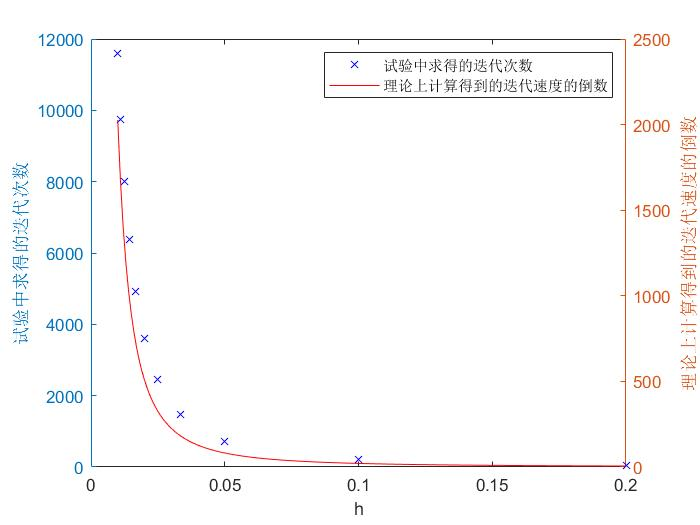
\includegraphics[scale=.5]{jacobivarh.jpg}
\caption{收敛速度和迭代次数随$h$变化情况} \label{jacobivarh}
\end{figure}

\section{MATLAB代码}
(1)雅可比迭代法
\begin{lstlisting}
clear,clc;
h = 0.1;
N = 1 / h;
epsilon = 10^(-6);
C = diag(ones(N - 2,1),1) + diag(ones(N - 2,1),-1);
L_h = zeros((N - 1) * (N - 1),(N - 1) * (N - 1));
for i = 1:N - 1
    L_h((N - 1) * (i - 1) + 1:(N - 1) * i,(N - 1) * (i - 1) + 1:(N - 1) * i) = 4 * eye(N - 1) - C;
end
for i = 1:N - 2
    L_h((N - 1) * (i - 1) + 1:(N - 1) * i,(N - 1) * i + 1:(N - 1) * (i + 1)) = -eye(N - 1);
    L_h((N - 1) * i + 1:(N - 1) * (i + 1),(N - 1) * (i - 1) + 1:(N - 1) * i) = -eye(N - 1);
end
f_h = zeros((N - 1) * (N - 1),1);
for j = 1:N - 1
    for i = 1:N - 1
        f_h((N - 1) * (j - 1) + i) = f(h * i,h * j);
    end
end
tic
D = eye((N - 1) * (N - 1)) .* L_h;% diagonal matrix of L_h
L = -(L_h - triu(L_h));% lower triangle matrix of L_h
U = -(L_h - tril(L_h));% upper triangle matrix of L_h
b = h^2 * f_h;
J = eye((N - 1) * (N - 1)) - D \ L_h;% Jacobi matrix
f1 = D \ b;
k = 0;% iteration times
u_h_k = ones((N - 1) * (N - 1),1);
u_h_past = zeros((N - 1) * (N - 1),1);
while norm(u_h_k - u_h_past,Inf) > epsilon
    k = k + 1;
    u_h_past = u_h_k;
    u_h_k = J * u_h_past + f1;
end
toc
u_star = zeros((N - 1) * (N - 1),1);% precise solution
for j = 1:N - 1
    for i = 1:N - 1
        u_star((N - 1) * (j - 1) + i) = sin(pi * h * i) * sin(pi * h * j);
    end
end
k
norm(u_h_k - u_star,1)
norm(u_h_k - u_star,2)
norm(u_h_k - u_star,Inf)
function y = f(x,y)
    y = 2 * pi^2 * sin(pi * x) * sin(pi * y);
end
\end{lstlisting}
(2)赛德尔迭代法
\begin{lstlisting}
clear,clc;
h = 0.1;
N = 1 / h;
epsilon = 10^(-6);
C = diag(ones(N - 2,1),1) + diag(ones(N - 2,1),-1);
L_h = zeros((N - 1) * (N - 1),(N - 1) * (N - 1));
for i = 1:N - 1
    L_h((N - 1) * (i - 1) + 1:(N - 1) * i,(N - 1) * (i - 1) + 1:(N - 1) * i) = 4 * eye(N - 1) - C;
end
for i = 1:N - 2
    L_h((N - 1) * (i - 1) + 1:(N - 1) * i,(N - 1) * i + 1:(N - 1) * (i + 1)) = -eye(N - 1);
    L_h((N - 1) * i + 1:(N - 1) * (i + 1),(N - 1) * (i - 1) + 1:(N - 1) * i) = -eye(N - 1);
end
f_h = zeros((N - 1) * (N - 1),1);
for j = 1:N - 1
    for i = 1:N - 1
        f_h((N - 1) * (j - 1) + i) = f(h * i,h * j);
    end
end
tic
D = eye((N - 1) * (N - 1)) .* L_h;% diagonal matrix of L_h
L = -(L_h - triu(L_h));% lower triangle matrix of L_h
U = -(L_h - tril(L_h));% upper triangle matrix of L_h
b = h^2 * f_h;
G = (D - L) \ U;% Jacobi matrix
f1 = (D - L) \ b;
k = 0;% iteration times
u_h_k = ones((N - 1) * (N - 1),1);
u_h_past = zeros((N - 1) * (N - 1),1);
while norm(u_h_k - u_h_past,Inf) > epsilon
    k = k + 1;
    u_h_past = u_h_k;
    u_h_k = G * u_h_past + f1;
end
toc
u_star = zeros((N - 1) * (N - 1),1);% precise solution
for j = 1:N - 1
    for i = 1:N - 1
        u_star((N - 1) * (j - 1) + i) = sin(pi * h * i) * sin(pi * h * j);
    end
end
k
norm(u_h_k - u_star,1)
norm(u_h_k - u_star,2)
norm(u_h_k - u_star,Inf)
function y = f(x,y)
    y = 2 * pi^2 * sin(pi * x) * sin(pi * y);
end
\end{lstlisting}
(3)超松弛迭代法
\begin{lstlisting}
clear,clc;
h = 0.1;
N = 1 / h;
epsilon = 10^(-6);
omega = 1.2;
C = diag(ones(N - 2,1),1) + diag(ones(N - 2,1),-1);
L_h = zeros((N - 1) * (N - 1),(N - 1) * (N - 1));
for i = 1:N - 1
    L_h((N - 1) * (i - 1) + 1:(N - 1) * i,(N - 1) * (i - 1) + 1:(N - 1) * i) = 4 * eye(N - 1) - C;
end
for i = 1:N - 2
    L_h((N - 1) * (i - 1) + 1:(N - 1) * i,(N - 1) * i + 1:(N - 1) * (i + 1)) = -eye(N - 1);
    L_h((N - 1) * i + 1:(N - 1) * (i + 1),(N - 1) * (i - 1) + 1:(N - 1) * i) = -eye(N - 1);
end
f_h = zeros((N - 1) * (N - 1),1);
for j = 1:N - 1
    for i = 1:N - 1
        f_h((N - 1) * (j - 1) + i) = f(h * i,h * j);
    end
end
tic
D = eye((N - 1) * (N - 1)) .* L_h;% diagonal matrix of L_h
L = -(L_h - triu(L_h));% lower triangle matrix of L_h
U = -(L_h - tril(L_h));% upper triangle matrix of L_h
b = h^2 * f_h;
L_omega = (D - omega * L) \ ((1 - omega) * D + omega * U);%Jacobi matrix
f1 = omega * ((D - omega * L) \ b);
k = 0;% iteration times
u_h_k = ones((N - 1) * (N - 1),1);
u_h_past = zeros((N - 1) * (N - 1),1);
while norm(u_h_k - u_h_past,Inf) > epsilon
    k = k + 1;
    u_h_past = u_h_k;
    u_h_k = L_omega * u_h_past + f1;
end
toc
u_star = zeros((N - 1) * (N - 1),1);% precise solution
for j = 1:N - 1
    for i = 1:N - 1
        u_star((N - 1) * (j - 1) + i) = sin(pi * h * i) * sin(pi * h * j);
    end
end
k
norm(u_h_k - u_star,1)
norm(u_h_k - u_star,2)
norm(u_h_k - u_star,Inf)
function y = f(x,y)
    y = 2 * pi^2 * sin(pi * x) * sin(pi * y);
end
\end{lstlisting}
\end{document}
